
\sys's implementation complements Apache HBase with transaction processing. 
It exploits HBase to store both  application data and the CT metadata. 
HBase, the TMs, and Zookeeper are all deployed on separate dedicated machines.

In large-scale deployments, HBase tables are  sharded (partitioned) into multiple \emph{regions}.
Each region is managed by a \emph{region server}; one server may serve multiple regions. HBase 
is deployed on top of Hadoop Distributed Filesystem (HDFS), which provides the basic abstraction 
of scalable and reliable storage. HDFS is replicated 3-fold in all the settings described below. 

Section~\ref{sec:prod} presents performance statistics obtained in \sys's 
production deployment, focusing on the end-to-end application-level overhead introduced 
by transaction processing. Section~\ref{sec:synthetic} further zooms in on the TM scalability
under very high loads.
%, via multiple benchmarks. 
%Since the transactions' access to application data is independent of \sys's design, 
%we focus the remaining evaluation, in Section~\ref{sec:thpt}, on benchmarking the TM.

\subsection{End-to-end performance in production}
\label{sec:prod}

We present statistics of \sys's use in a production deployment of Sieve -- Yahoo's
content management system. 
Sieve digests streams of documents from multiple sources, processes them, and indexes 
the results for use in search and personalization applications. Each document 
traverses a pipeline of  tasks, either independently or as part of a mini-batch. 
A task is an  ACID processing unit, framed as a transaction. It typically reads 
one or more data items generated by  preceding tasks, performs some computation, 
and writes one or more artifacts back. 

Sieve scales across task pipelines that serve multiple products,  performing tens of thousands 
of tasks per second on multi-petabyte storage. All  
are powered by a single \sys\ service, with the CT sharded across $10$ regions
managed by $5$ region servers.  
Sieve is throughput-oriented, and favors  scalability over transaction latency. 

\comment{
Table~\ref{table:workload} summarizes the compute and I/O footprint of selected Sieve tasks
within a particular Sieve instance that processes web content, performing tens of thousands 
of tasks per second on multi-petabyte storage. 

\begin{table}[htb]
\centering
\begin{tabular}{| l | l | l |}
\hline
Task	 &  Compute   & \# KV-store \\
         &  time (avg) & accesses (avg)\\
\hline
Document inversion		& 650ms	 & 13 \\
Duplicate detection		& 1.4ms     & 8	\\
Out-link processing		& 35ms      & 3	\\
In-link processing		& 150ms	 & 6	\\
Streaming to runtime		& 2050ms  & 5	\\
\hline
\end{tabular}
\caption{{\bf Production workload.} Task characteristics in a production Sieve deployment powered by \sys.}
\label{table:workload}
\end{table}
}

\begin{figure}[htb]
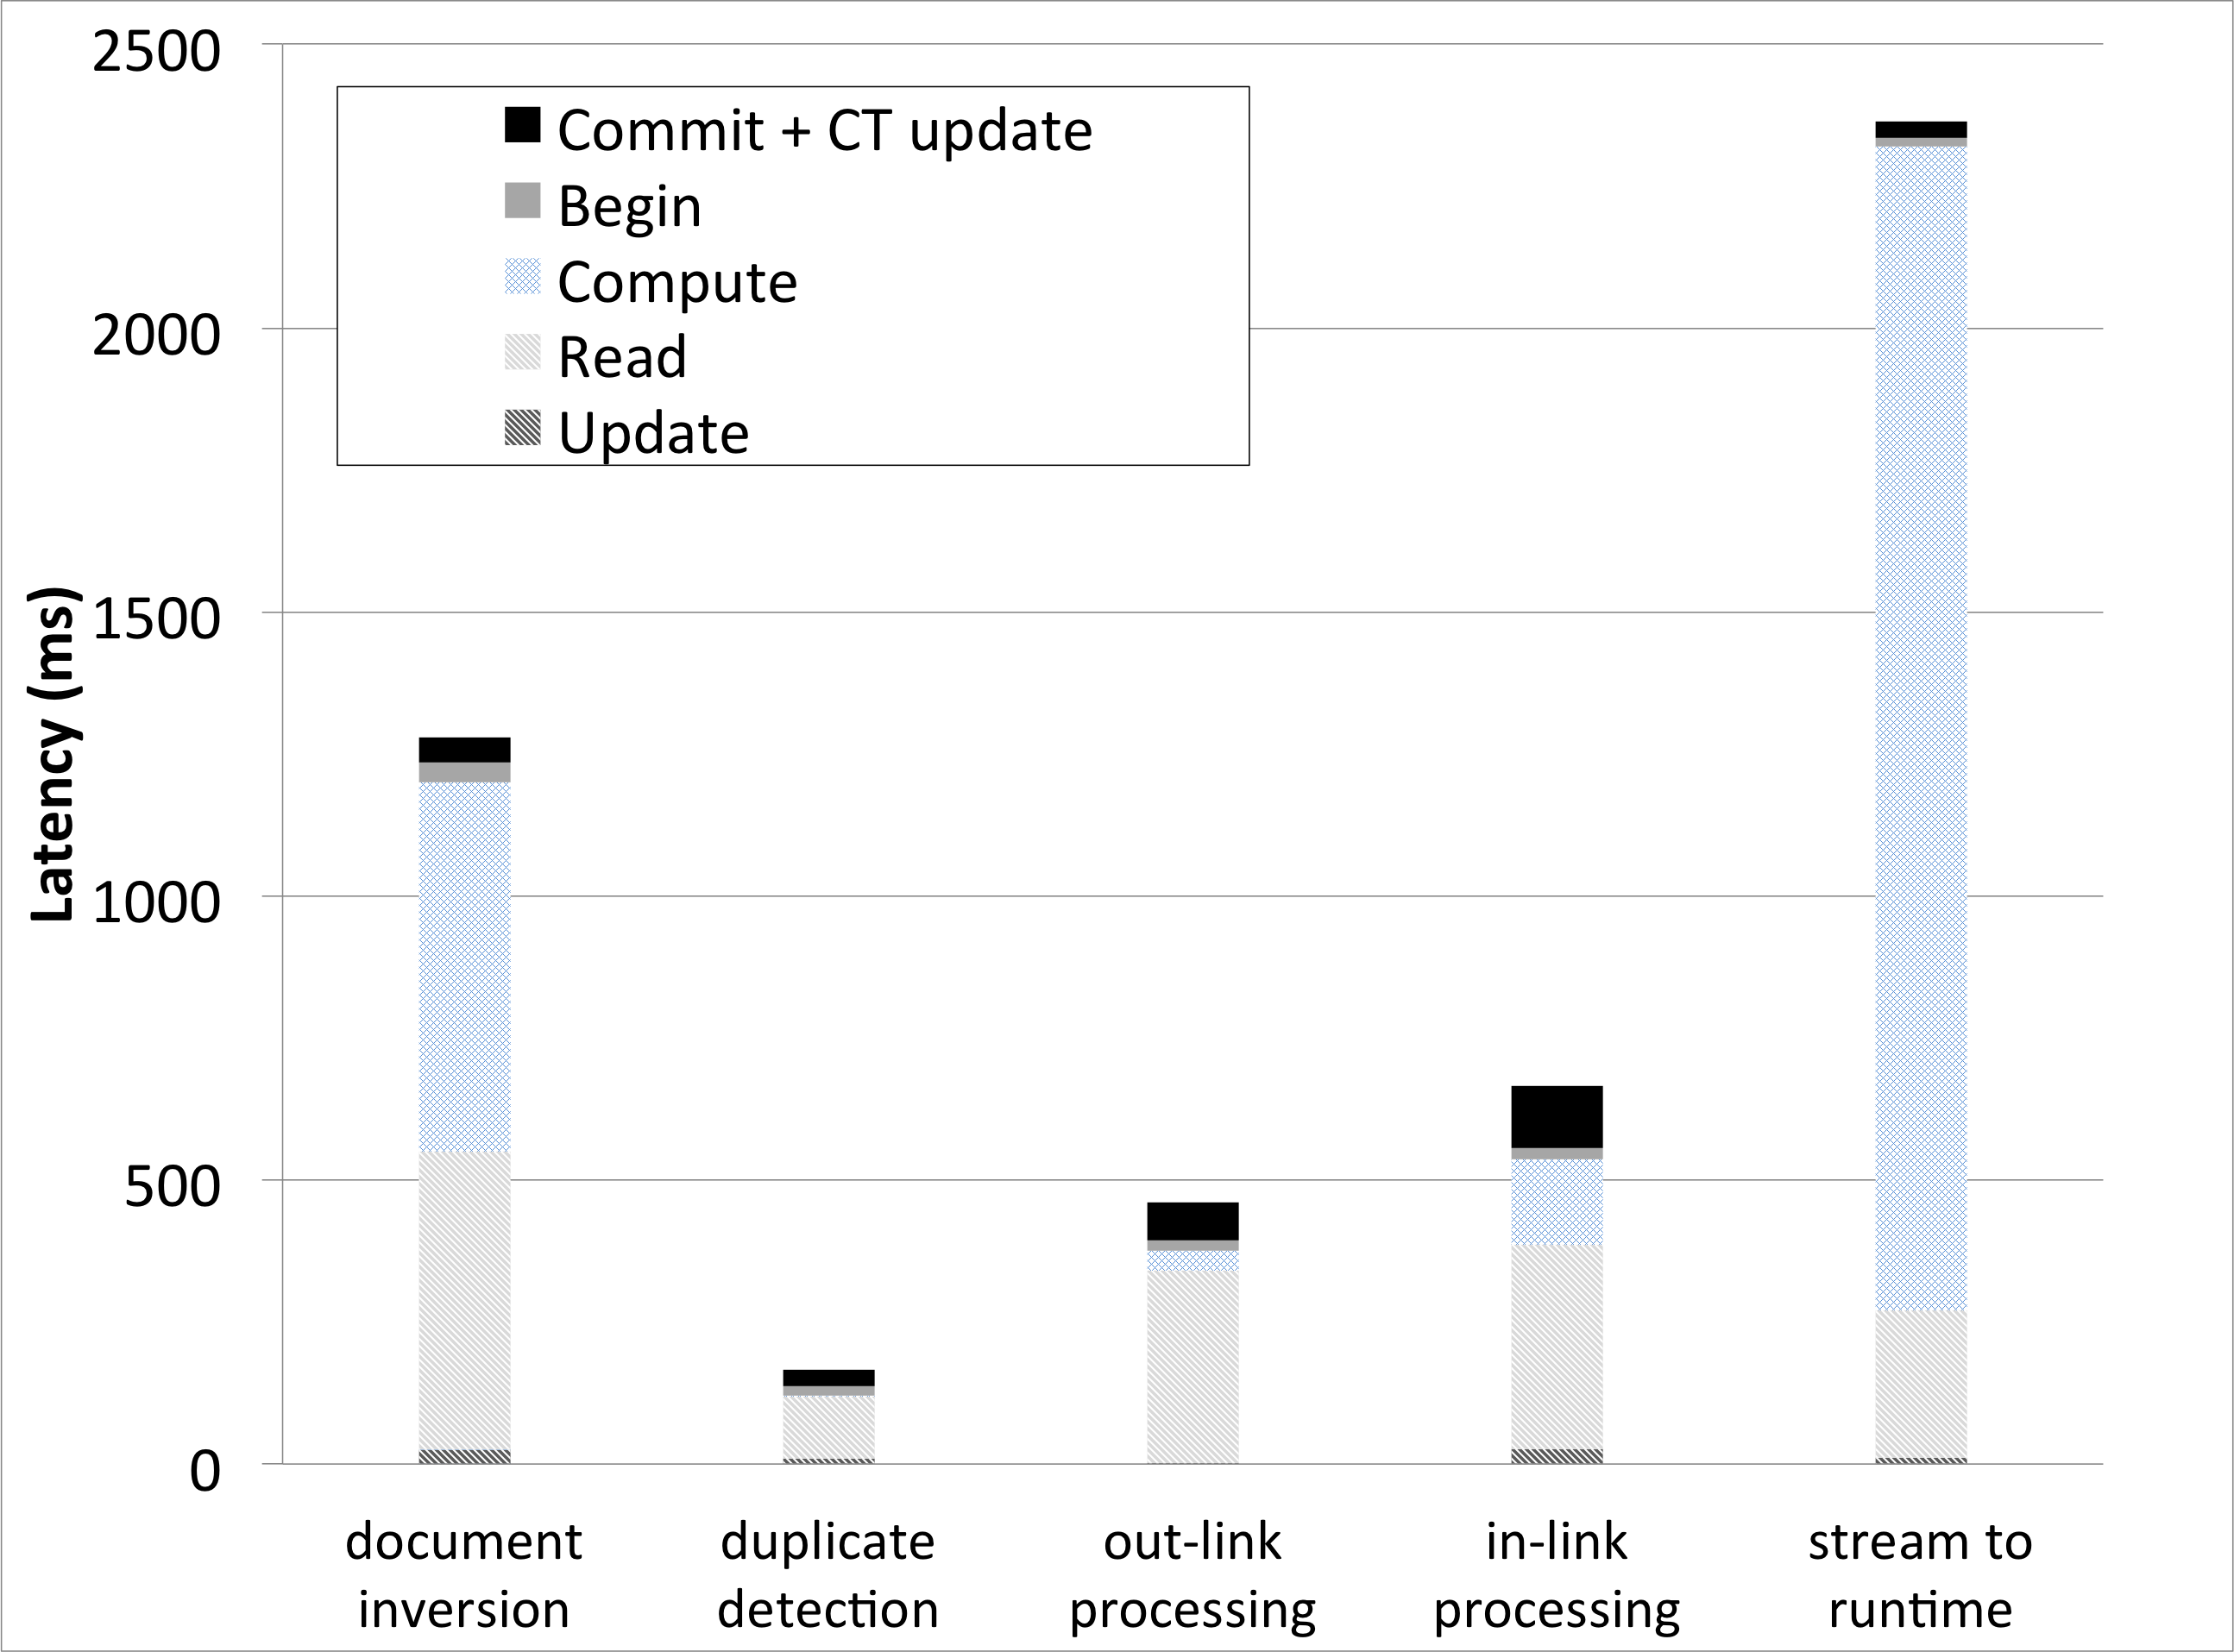
\includegraphics[width=\figw]{Latency-Sieve.png}
\caption{{\bf Transaction latency breakdown in production deployment of \sys\ in Sieve.} The top two components represent 
transaction management overhead.
}
\label{fig:sieve_latency}
\end{figure}

Figure~\ref{fig:sieve_latency} presents statistics gathered for five selected Sieve tasks. 
For each task, we present its average latency broken down to components --
HBase access (two bottom components in each bar), compute time, and the TM's begin and commit  (top two components). 
In this deployment, \sys\ updates the commit fields synchronously upon commit, that is, commit returns only 
after the commit fields of the transaction's write-set have been updated. 
%(the additional latency is reflected in the top component in each bar). 
\remove{
This approach prevents contention on data items produced 
by some task and immediately consumed by the ensuing  task in the pipeline. 
}
Note that since a begin request waits for all transactions with smaller $txids$ to commit, its processing
latency is similar to that of a commit operation, minus the time commit takes to update the commit fields. 


We see that for tasks that perform significant processing and I/O,  like 
document inversion and streaming to index, 
\sys's latency overhead (for processing begin and commit) is negligible --  $2$--$6\%$ of the total transaction duration. 
In very short tasks such as duplicate detection and out-link processing, \sys\ accounts for up to roughly one third of the transaction latency.
%In more latency-sensitive applications, the latency can be further shortened by deferring the commit field updates to execute asynchronously.


The transaction abort rates observed in Sieve are negligible (around $0.002\%$). 
They stem from either transient HBase outages or 
write-write conflicts, e.g., concurrent in-link updates of extremely popular web pages.  

\subsection{TM microbenchmarks}
\label{sec:synthetic}

We now focus on TM performance. 
To this end, our microbenchmarks  invoke only the TM's begin and commit APIs, and do not access actual data.
We run both the TM and HBase (holding the CT) on industry-standard 8-core 
Intel Xeon E5620 servers with 24GB RAM and 1TB magnetic drive. The interconnects  are 1Gbps Ethernet.


We generate workloads in which transaction write-set sizes are distributed Zipf, i.e., follow a power-law ($Pr[X \geq x] = x^{-\alpha}$) 
with exponent values of $\alpha=1.2$, $\alpha=1.6$, and $\alpha=2$ (the smaller the heavier-tailed), cut-off at $256$ keys.
Each transaction's latency, (i.e., the time we wait after invoking its begin and before invoking its commit), is set to $5$ms per write. 
Note that read-sets are not sent to the TM and hence their size is immaterial.

We note that key selection affects \emph{real} conflicts: if the written keys are drawn from a heavy-tailed distribution, then two concurrent 
transactions are likely to update the same key, necessitating one of them to abort. Since this is an artifact of the workload, which is unaffected
by our system design, we attempt to minimize this phenomenon in our experiments. We therefore uniformly sample 64-bit integers
for the key hashes. Recall that our experience in production shows that real conflicts are indeed rare.


We begin by evaluating scalability, which is our principal design goal.
The TM throughput is constrained by two distinct resources -- the storage access required for persisting commits in the CT, and
the compute resources used for conflict detection.
These resources scale independently: the former, evaluated in Section~\ref{ssec:ct-scale}, scales out across multiple HBase region servers, 
whereas the latter scales up on multi-core hardware, and is studied in Section~\ref{ssec:mc-scale}.
Section~\ref{ssec:latency} then evaluates the throughput-latency tradeoff that \sys\ exhibits when using a single region server.
Finally, in Section~\ref{sec:ha-eval}, we exercise \sys's high-availability mechanism. 

\subsubsection{Commit table scalability} 
\label{ssec:ct-scale}

\begin{figure}
\centerline{
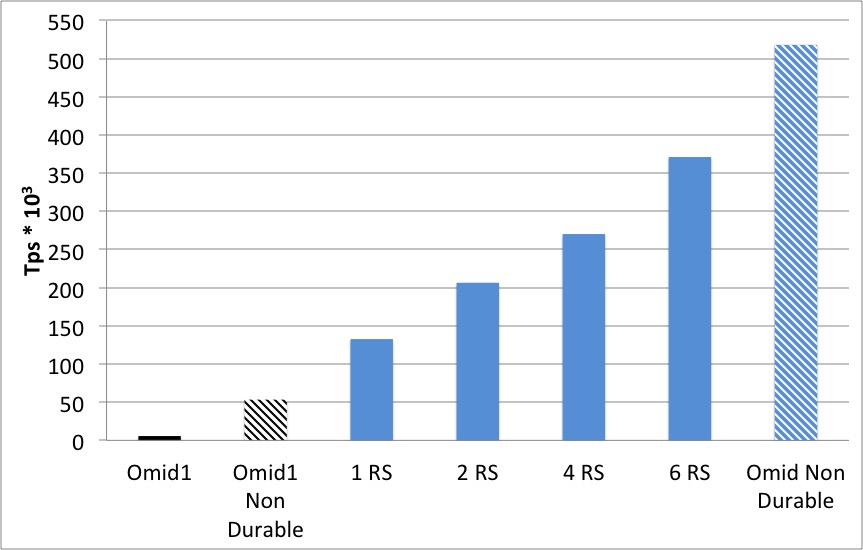
\includegraphics[width=\figw]{CT+Omid1.png}
}
\caption{{\bf Scalability of \sys's CT updates with the number of HBase region servers, and comparison with Omid1.} Non-durable versions do not persist transactions and thus provide upper bounds on throughput under perfect storage scaling. 
%\sys\ uses $4$ writer threads and 2K transaction batches. 
}
\label{fig:ct_thpt}
\end{figure}


Since the commit records are fixed-length (two 64-bit integers), the CT performance does not depend on transaction sizes, and 
so we experiment only with $\alpha=1.6$.
Recall that in order to optimize throughput, the TM batches writes to the CT and issues multiple batches in parallel. 
Experimentally, we found that the optimal number of concurrent CT writer threads is $4$, and  
the batch size that yields the best throughput is 2K transactions per writer. 

Figure~\ref{fig:ct_thpt} depicts \sys's commit rate as function of the number of HBase region servers,
which scales to almost 400K tps.
It further compares \sys's throughput to that of  Omid1~\cite{OmidICDE2014}, which, 
similarly to \sys, runs atop HBase, and uses a centralized TM. 
%and is configured the same way as \sys.  
% with 4 writer threads at the TM side and 6 region servers at the HBase side. 
It is worth noting that even in the single-server configuration, \sys\ outperforms
Omid1  by more than 25x. This happens because upon each begin request, Omid1 sends to the client a large amount 
of information (equivalent to the combination of \sys's CT and the in-memory conflict detection table). 
%Under the studied transaction rates, 
This saturates the CPU and network resources. 

The ``non-durable'' bars -- leftmost and second from the right -- represent experiments where commits are not persisted 
to stable storage. In \sys\ this means forgoing the write to the CT, whereas in Omid1 it means disabling the write to BookKeeper
in which the system stores its commit log.  
These results provide upper bounds on the throughput that can be obtained with perfect storage scaling in both systems. 
\sys\ peaks at 518K transactions per second, whereas Omid1 peaks at 50K. 


\subsubsection{Conflict detection scalability} 
\label{ssec:mc-scale}



\begin{figure*}[tb]
\begin{subfigure}{\columnwidth}
\centerline{     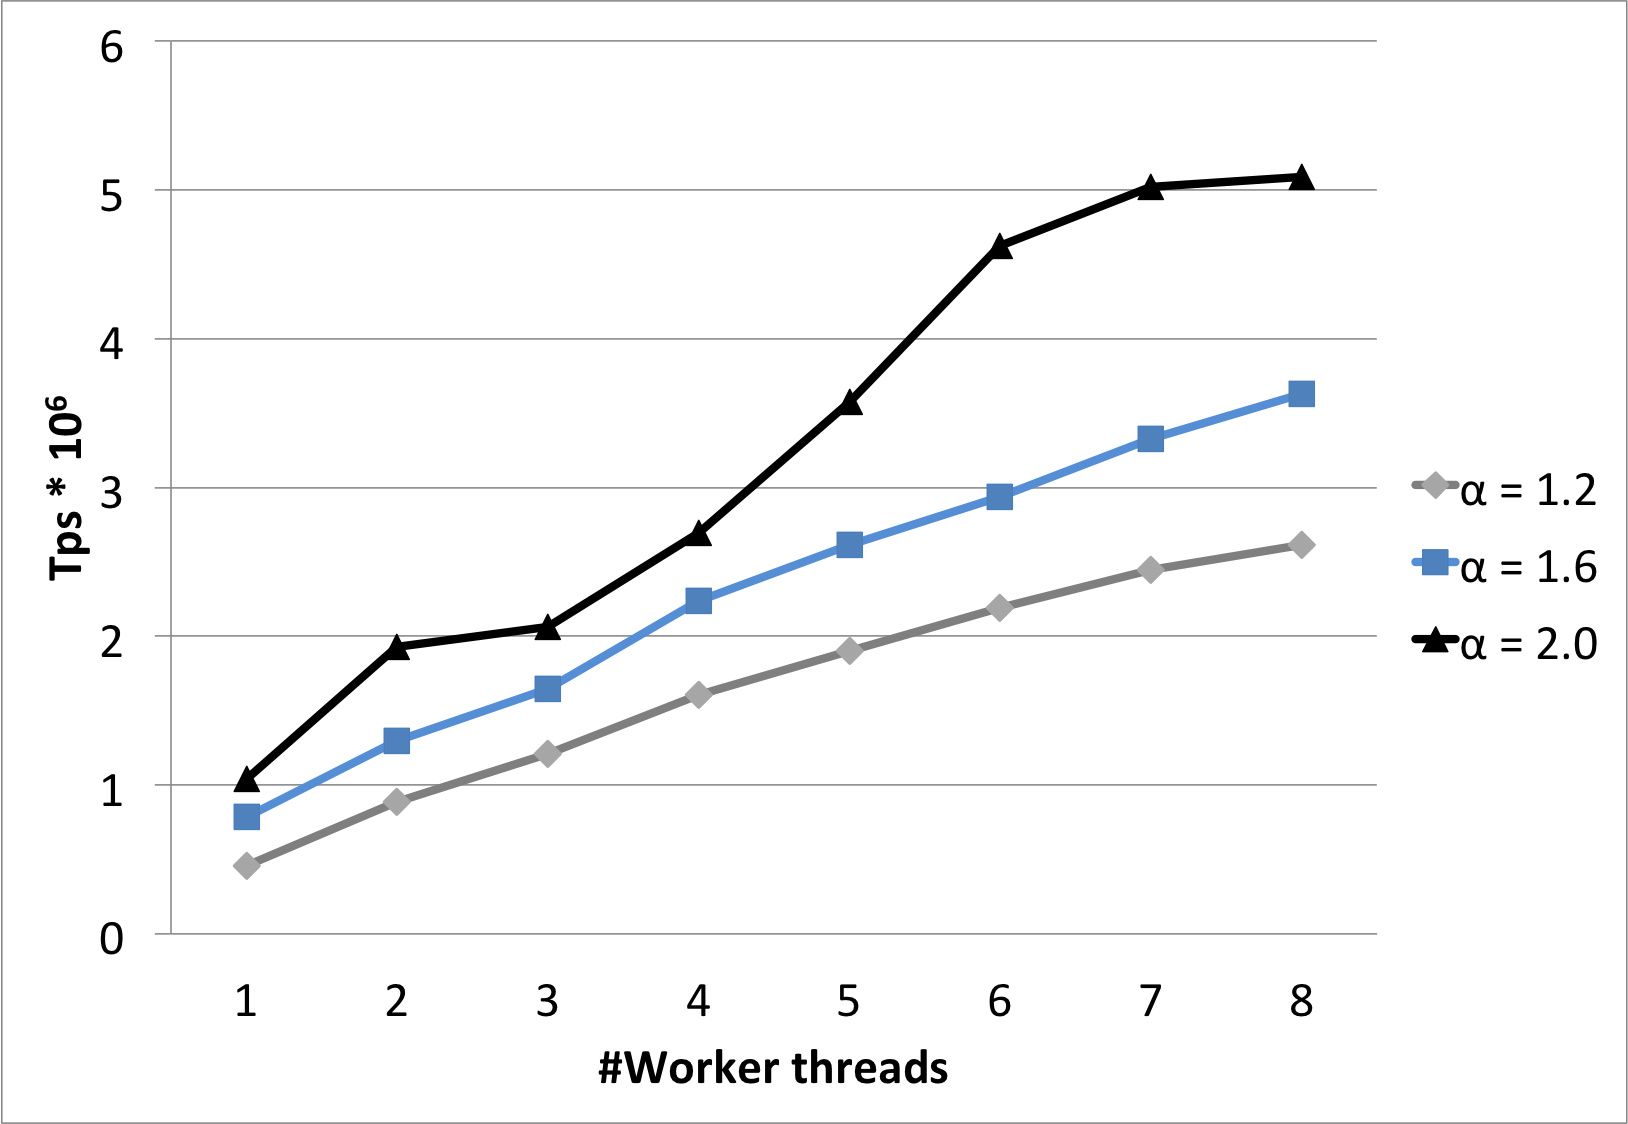
\includegraphics[width=\columnwidth, height=5.25cm]{CDPerf.png} }
	\hspace{0.25cm}
    \caption{Conflict detection scalability}
    \label{fig:1}
  \end{subfigure}
\hspace{\columnsep}
\begin{subfigure}{\columnwidth}
\centerline{      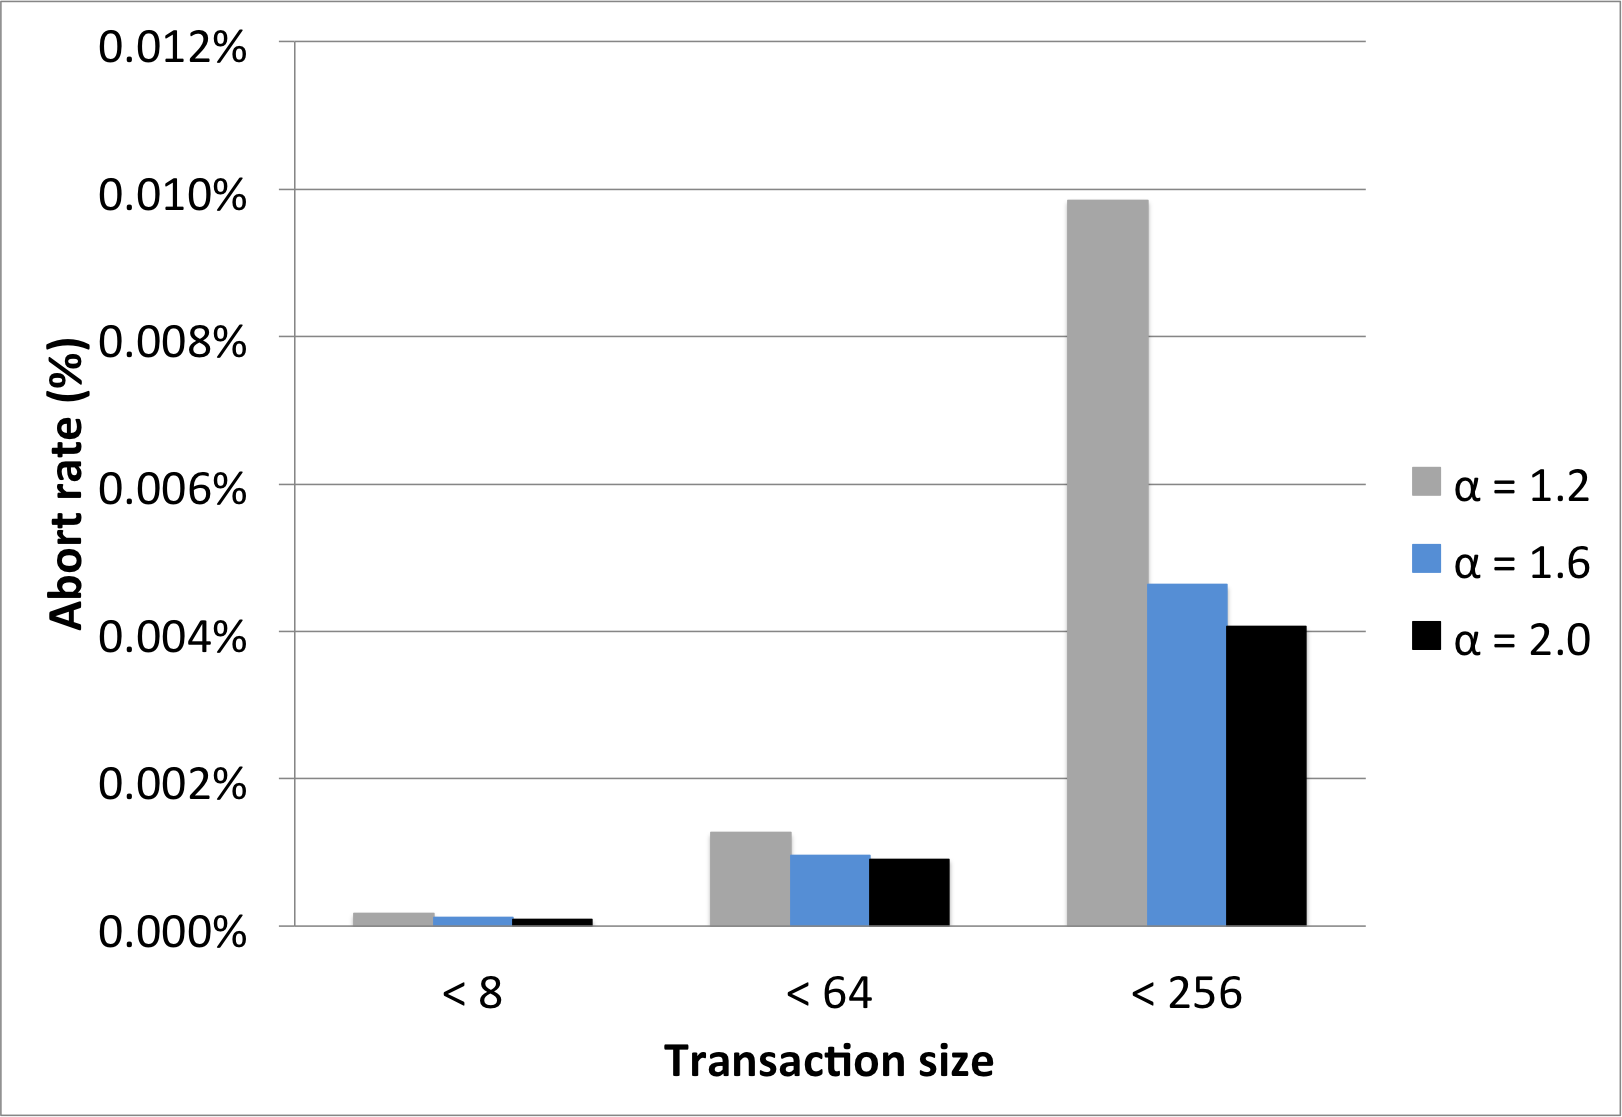
\includegraphics[width=\columnwidth, height=5.25cm]{CDAbort.png} }
	\hspace{0.25cm}
    \caption{Conflict detection false abort rate}
    \label{fig:2}
  \end{subfigure}
\caption{{\bf Conflict detection scalability and false abort rate.} Transaction write-set sizes are distributed power-law ($Pr[X \geq x] = x^{-\alpha}$) 
with exponent values of $\alpha=1.2$, $\alpha=1.6$, and $\alpha=2$ (the smaller the 
heavier-tailed); the key hashes are $6$4-bit integers, uniformly sampled to avoid real conflicts whp; transaction latency is $5$ms per write.}
% 2 plots side by side
\label{fig:cd_perf}
\end{figure*}

In the experiment reported  above, the conflict detection algorithm is evaluated as part of the system.
There, the commit table I/O is the bottleneck, and the conflict detection process can keep up with the pace
of four I/O threads even when running sequentially, i.e., in a single thread. 

We next focus on scale-up of this component running by itself using $1$ to $8$ threads, in order to study its potential scalability in even larger configurations.
The experiment employs a conflict table of 128M 64-bit integers (1G total size). The bucket size is $32$ integers, i.e., the table is 4M buckets big.  

\remove{
When testing the conflict detection component, transaction size is of essence: long transactions are more likely than short ones to
incur spurious aborts due to turnover in hash  buckets. 
We consider three power-law exponent values -- $\alpha=1.2$, $\alpha=1.6$, and $\alpha=2$.
}

Figure~\ref{fig:cd_perf}(a) illustrates the processing rate.
As expected processing shorter transactions (a bigger  $\alpha$) is faster.
%for the three values of $\alpha$. The latency of processing a single commit request is proportional to the transaction size, 
% therefore the throughput is larger for a bigger  $\alpha$ (lighter tail). 
The rate scales to 2.6M transactions per second for $\alpha=1.2$, and to 5M for 
$\alpha=2$. Note that exercising such high throughput in a complete system would require an 
order of magnitude faster network to sustain the request/response packet rate.    
Clearly the TM's compute aspect is far from being a bottleneck.

% Recall that the CD is an imperfect filter with no false negatives. 
Finally, we analyze the false abort rate. (The uniform sampling of key hashes and relatively 
short transaction latencies render real collisions unlikely, hence all aborts 
are deemed false). The overall abort rate is negligibly small. In 
Figure~\ref{fig:cd_perf}(b) we  zoom-in
 on  transactions clustered into three buckets: shorter than $8$ writes, $8$ to $63$ writes, and 
$64$+ writes.
The worst abort rate is below $0.01\%$. It occurs, as expected, for long transactions in the 
most heavy-tailed distribution.  Further reduction of the false abort rate would require 
increasing the table size or using multiple hashes (similarly to Bloom filters). 

\remove{
The implementation is extremely memory-intensive, benefitting little from hardware caches since there is no locality of access 
among requests and keys. Using a much smaller table (1M 64-bit integers)  leads to about 
30\% increase in throughput because the entire table fits into the L2 cache in this case. 
However, at the huge commit rates exercised by protocol, the lifetime of a particular timestamp
in a bucket becomes much smaller in this setting, leading to  loss of precision. Our experiments 
show that in this case, most of the long transactions would experience false aborts.
Therefore, this setting cannot be used in a real system without additional measures for mitigating
abort rates of long transactions.  
}

\subsubsection{Latency-throughput tradeoff} 
\label{ssec:latency}

We now examine the impact of load on  TM access latency with a single region server managing the CT. We use here $\alpha= 1.6$. 
For every given system load, the batch size is tuned for optimal latency:
under light load, no batching is employed, (i.e., commits are written one at a time), whereas
under high load, we use batches of 10K. 

Figure~\ref{fig:omid_latency} reports the average
client-side latency of commit operations, 
broken down to three components: (1) network round-trip delay and conflict detection, which are negligible, and 
do not vary with the load or batch size;
(2) HBase CT write latency, which increases with the batch size; and (3) queueing delay at the TM, which increases with the load.
Begin latency is similar, and is therefore omitted.
We increase the load up to $70$K transactions per second, after which the latency becomes excessive; 
to exceed this throughput, one may use multiple region servers as in the experiment of Section~\ref{ssec:ct-scale}. 

\begin{figure}[h!]
\centerline{
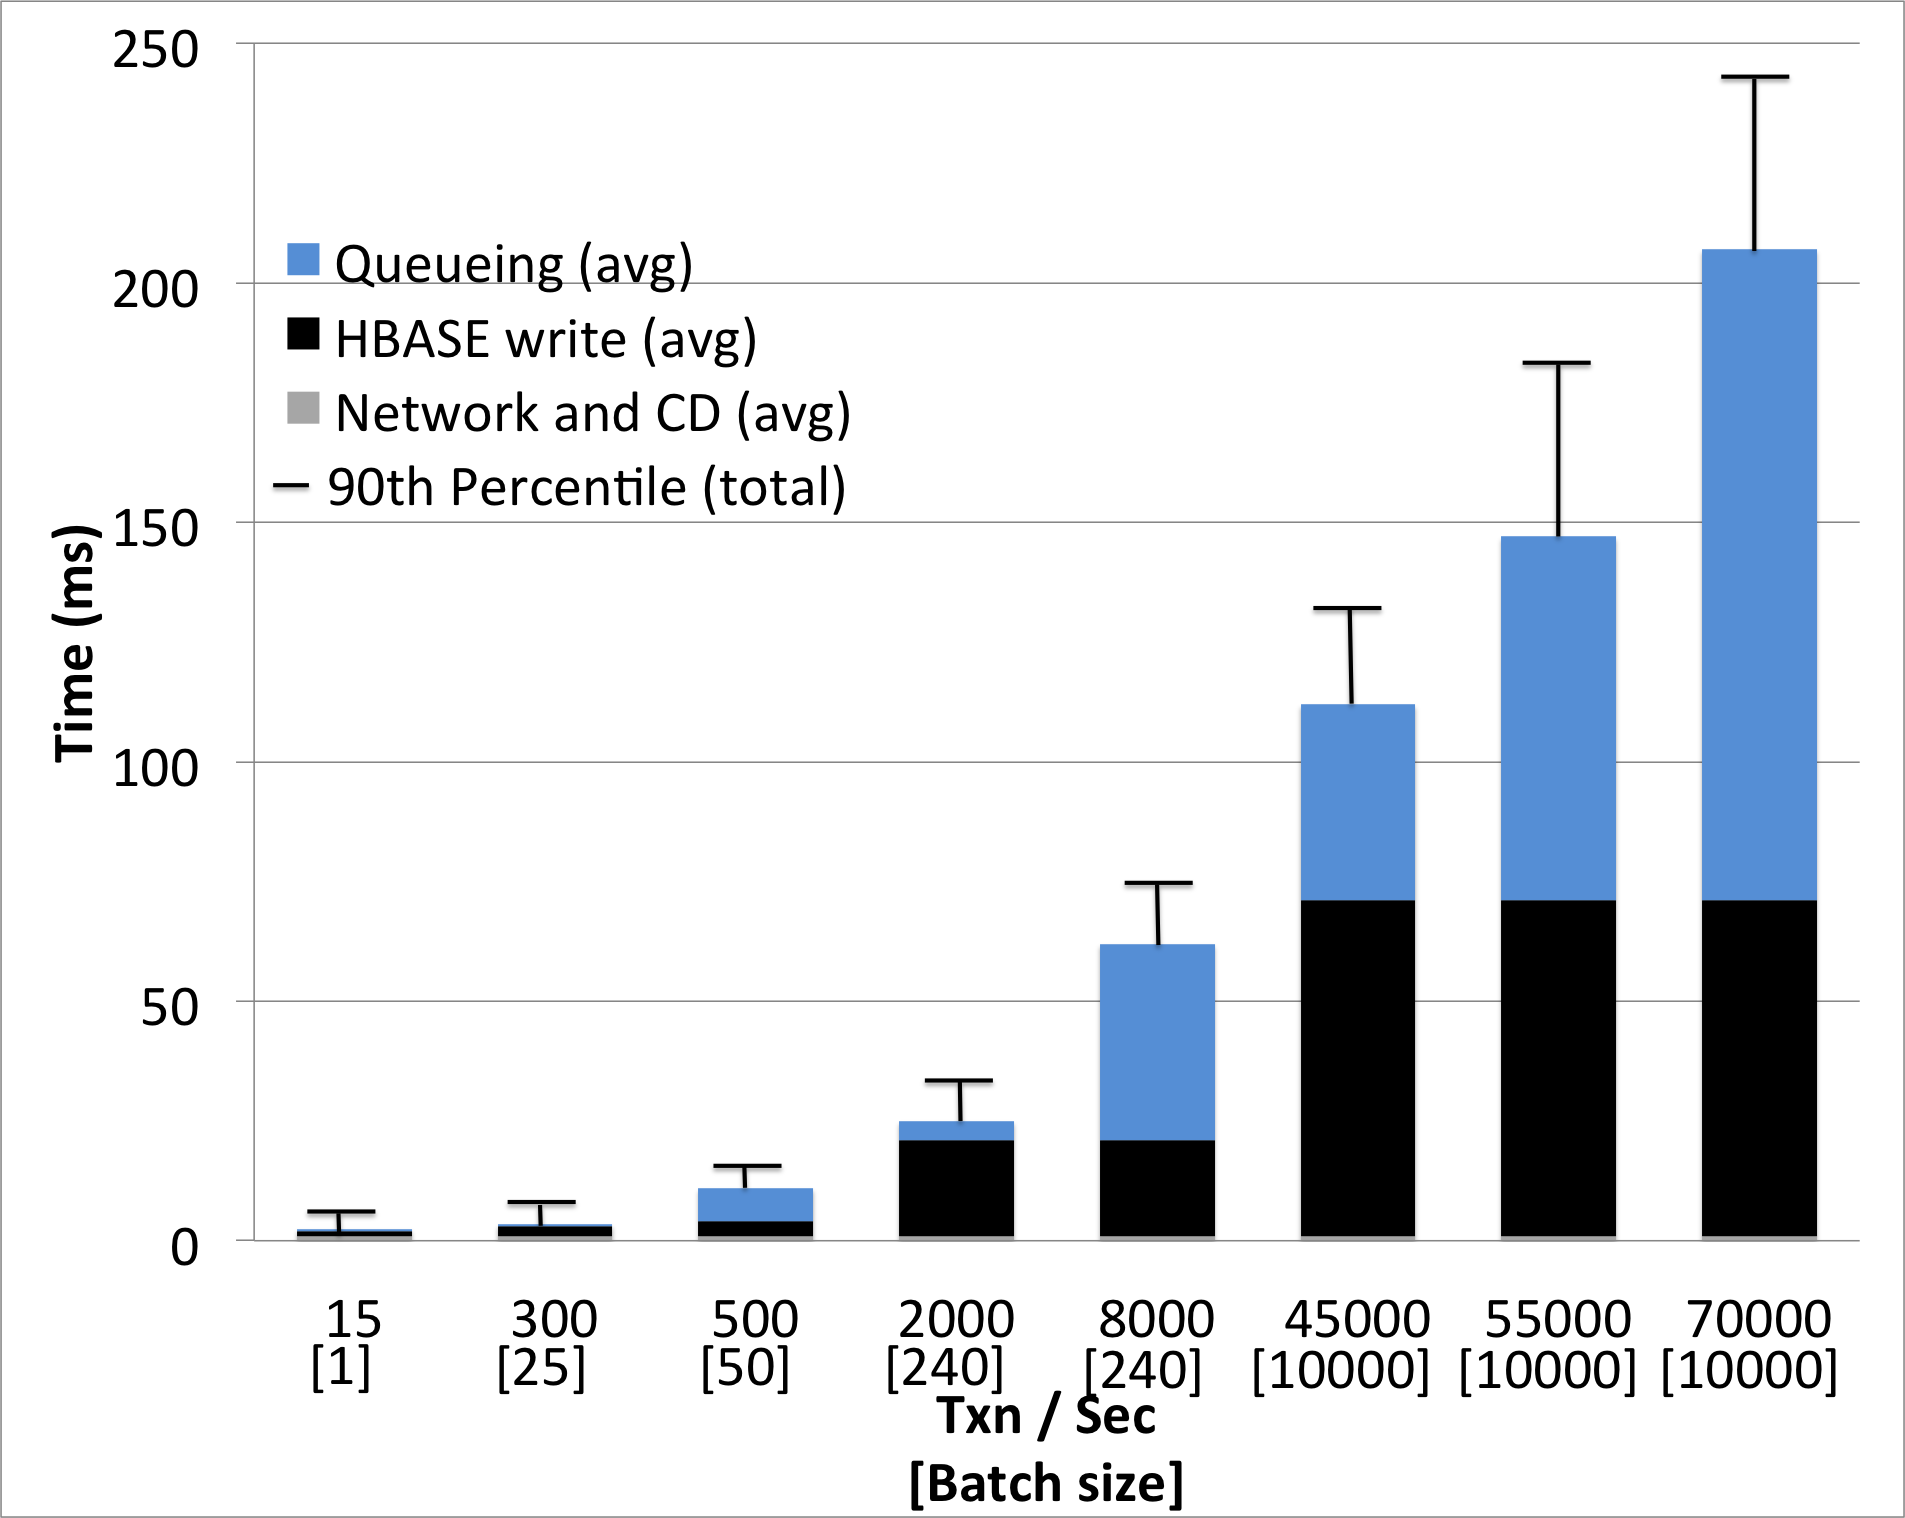
\includegraphics[width=0.975\columnwidth]{Latency-Omid.png}
}
\caption{{\bf \sys\ throughput vs.\ latency.} Client-perceived commit latency (average broken down and $90\%$ of total); single region server; power-law transaction sizes  with $\alpha=1.6$; batch sizes optimized for minimum latency (in square brackets below each bar).
}
\label{fig:omid_latency}
\end{figure}

\begin{figure}[h!]
\centerline{
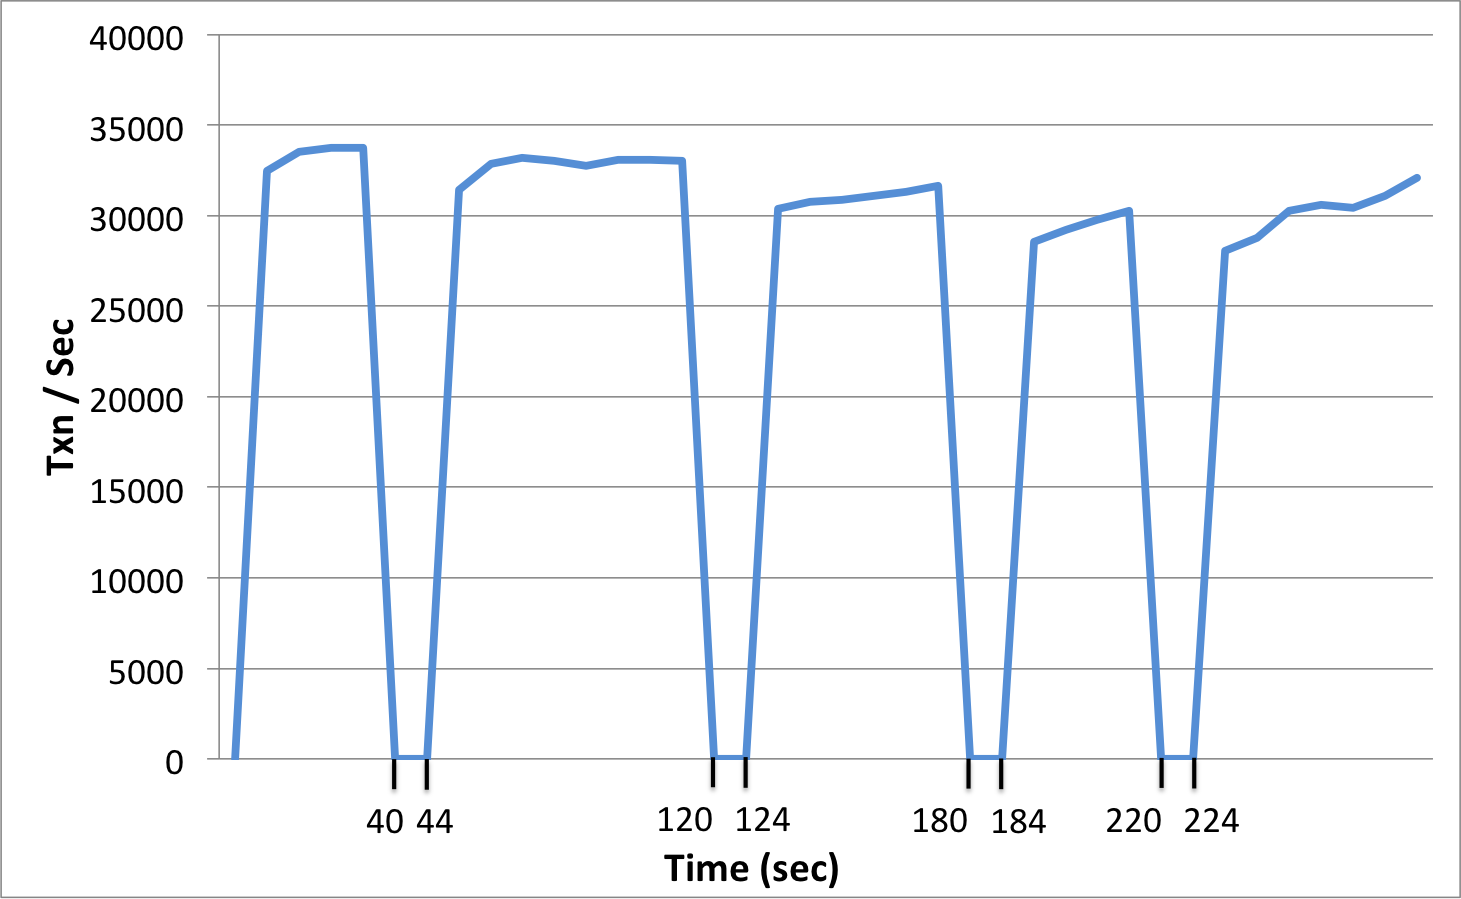
\includegraphics[width=\columnwidth]{HA.png}
}
\caption{{\bf \sys\ throughput with four failovers}; recovery takes around $4$ seconds. }
\label{fig:ha_recovery}
\end{figure}


\subsubsection{High availability}
\label{sec:ha-eval}


Finally, we exercise the high-availability mechanism. As long as the primary TM does not fail, HA induces negligible overhead. 
We now examine the system's recovery following a primary TM failure.  
The failure detection timeout is $\delta=1$ sec.
Figure~\ref{fig:ha_recovery} depicts  the system throughput over time, where the primary TM is forcefully shut down 
after  $40$ sec, is then allowed to recover, and the new primary (original backup) is shut down after $120$ sec. 
The primary is shut down two more times at $180$ and $220$ sec; the failover completes within $4$ sec.




